\chapter{Implementation} \label{implementation}

For this project I implemented the design as described in the previous chapter.
It is a command line application that takes a source code file as input and
performs semantic analysis on its \gls{ast}. I chose to write my implementation
using the Rust programming language. It is a memory safe language that leverages
the LLVM backend for highly optimized code. This makes it easy to write
robust and performant code. It additionally has very good parallel programming
facilities and an extensive software ecosystem that makes it ideal for this kind
of project. 

\begin{listing}[t]
\begin{minted}[linenos]{text}
fn factorial[n: int] {
    if n == 0 {
        return 1;
    } 

    return (n * factorial(n - 1));
}
\end{minted}
\caption{Factorial in the test language.}
\label{lst:factorial_example}
\end{listing}

Due to a generic lexical and syntatic analysis implementation, as described in the previous chapter,
the compiler supports parsing JSON aswell as a bespoke test language with syntax similar to Rust,
shown in Listing \ref{lst:factorial_example} and \ref{lst:json_example}.

Section \ref{structure} provides an explanation of the programs structure and implementation
details.
\newline \newline
Section \ref{outputs_and_visualizations} shows example outputs from the compiler as well as some
graphs which proved useful during debugging the individual compilation stages.
\newline \newline
Section \ref{dependancies} concludes with a description of the dependancies used and their purpose
in the implementation.

\section{Structure} \label{structure}

I will explain the implemention in the order of its execution. The program is divided into three
general stages: lexical, syntactic and semantic analysis. There are significant pre-processing
steps that need to happen prior to the core lexing and parsing algorithms, which can be computed at
compile time, but I nevertheless chose to do at runtime. The following section begins by describing
this pre-processing work that initializes some datastructures that are used later in the compiler.
The subsequent three sections describe the implementation of each of the compilation stages.

\subsection{Lexer Preprocessing}

In order for the compiler to support different languages, while sharing as much code as possible,
it is neccessary to generate datastructures that can be used by a generic lexer and parser
implemenentation. Furthermore, the datastructures required for bottom-up parsing are very difficult
to create without some form for automatic generation. Although a hand-written, language specific
implementation has significant optimisation potential, as shown by \cite{langdale_parsing_2019},
the focus of my implementation is to demonstrate the effectiveness of data-parallel compilation.
Single threaded optimisations that leverage the language or \gls{simd} instructions are sufficiently
orthogonal to this goal to put them outside the scope of the FYP. 

In order to for the lexer to work, a state transition table must be obtained. This is
done by firstly reading a reading a file that contains the mapping between the lexemes and
their corresponding regular expressions. An example of the syntax can be seen in listing
\ref{lst:json_lexical_grammar}. The \gls{ast} of each regular expression is then traversed and
converted into one, large joint \gls{nfa} graph using thompson's construction algorithm. This is
a classic algorithm that is described by \cite{aho_compilers_2006}, originally attributed to Ken
Thompson. It works by recursively breaking down the regex into simpler components and building
an \gls{nfa} for each component. The resulting NFA recognizes the same language as the original
regex. For my implementation I use an external library to parse the regex into an \gls{ast}. I then
traverse this \gls{ast}, building the \gls{nfa} as described by the algorithm

This graph is then turned into a \gls{dfa} through powerset construction. For this
algorithm I followed the steps outlined in wikipedia article on powerset construction
\citep{noauthor_powerset_2023}. It works by simulating an \gls{nfa} and interpreting the sets of
states reachable from each state in the \gls{nfa}, as the states of the \gls{dfa}. In other words,
it neccessary to simulate the \gls{nfa} and keep track of all states that the automaton could
reach after seeing an input, according to its nondeterministic choices. Each set of choices is then
converted into a corresponding state in the \gls{dfa}.

An example \gls{nfa} and \gls{dfa} for the JSON grammar is shown in figure \ref{fig:nfa} and figure
\ref{fig:dfa}, respectively. I implemented the graph traversals in both algorithms by keeping track
of a stack of nodes that have already been previously encountered. The \gls{dfa} can be tivially
turned into a state transition table by traversing it from its initial state and  taking note of
each pair of states connected by a transition. The parser similarly requires an operator precedence
table that must be computer generated due to its complexity.

\begin{listing}[t]
\begin{minted}[linenos]{json}
{
  "a": 100,
  "b": {
    "x": [
      100,
      "a"
    ]
  }
}
\end{minted}
\caption{Example of parsable JSON.}
\hrulefill
\label{lst:json_example}
\end{listing}

\subsection{Parser Preprocessing} 

The parser defined by \cite{barenghi_parallel_2015} is a standard operator
precedence algorithm that is modified to allow the parsing of non-terminals.
This parser requires that the structure of the language grammar follow certain
rules, as been defined in chapter \ref{design_parser}. A preliminary validation
of the grammar is performed to ensure that it conforms to these rules. It also
fixes any production rules with duplicate right-hand sides by creating new
production rules with new non-terminals in a way that keeps the resulting parse
tree structure predictable. After this validation step, the grammar is ready to
be parsed. Since this is an operator precedence parser, it additionally requires
an operator precedence table.

An operator precedence table can be derived by an algorithm that iterates over
the production rules of a grammar and determines the associativity of each
terminal symbol. 

\subsection{Lexical Analysis}

The lexer works by first splitting the input into equal sized chunks. 

\subsection{Syntactic Analysis}


\subsection{Semantic Analysis}

\section{Outputs} \label{outputs_and_visualizations}

The

\section{Dependencies} \label{dependancies}

Code dependencies in the Rust code ecosystem that are  available through the cargo package manager
are called crates. These crates are comparable to small, open source, third party libraries that can
easily be integrated into a rust project. In this section I mention the code dependencies I've used
in my implementation in order to illustrate what parts of my project were accomplished through the
use of third party code.

\subsection{Core}

\textbf{crossbeam} - Common data structures for implementing parallel systems.
This crate implements a concurrently accessible queue, skiplist and a
multi-producer, multi-consumer message passing channel. All of these data
structures are important for reliably sharing data across threads.
\newline\newline
\textbf{regex-syntax} - A crate for parsing standard regular expression syntax.
It provides a simple \gls{ast} that the lexer uses to read the mappings from
lexemes to regular expression patterns.
\newline\newline
\textbf{dot} - A crate that makes it easier to generate graphs in the dot
language. Its used to visualise the parse tree and \gls{ast}.
\gls{ast}.
\newline\newline
\textbf{criterion} - Reliable benchmarking facilities for testing the performance of the
compiler with differently sized inputs.

\subsection{Utility or Minor Contribution}
\textbf{tinyrand} - A lightweight implementation of random number
generation. It is used for creating unique IDs for bathes of work in the work
queue.
\textbf{serde} - Serialization and deserialization capabilities for transferring
code to and from the javascript runtime when running in the browser.
\newline\newline
\textbf{wasm-bindgen} - Macro's for easily creating bindings to javascript when
compiling to web assembly.
\newline\newline
\textbf{log, flexi\_logger ,wasm\-logger, console\_error\_panic\_hook} - Various
crates for logging to files as well as to the terminal, improved formatting and
correct logging when running in the browser.
\newline\newline
\textbf{simple-error} - A simple library for creating errors from error messages
instead of creating types for every error.

\subsection{Optimisation}
\textbf{memmap} - An interface for using linux's memmap syscall. Using memap to
read large files is  faster than using the standard read syscall.
\newline\newline
\textbf{bittyset} - A set implementation that uses a bit vector as a backing
store. This enables a compact representation as well as faster set operations in
the parser where sets of terminals and non-terminals are used.

\begin{figure}[t]
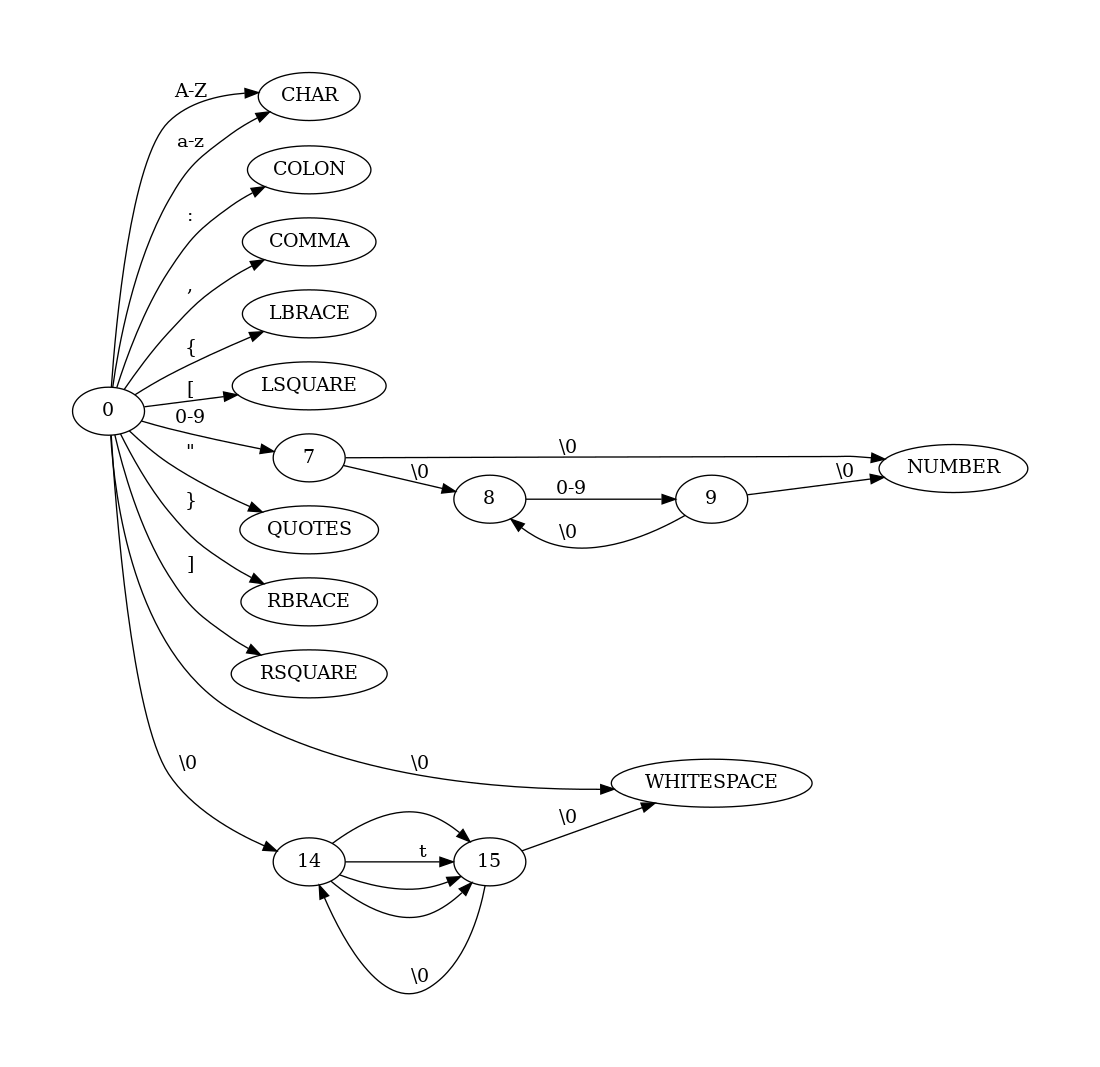
\includegraphics[width=\linewidth]{images/nfa.png}
\caption{NFA of the lexical grammar}
\label{fig:nfa}
\end{figure}

\begin{figure}[t]
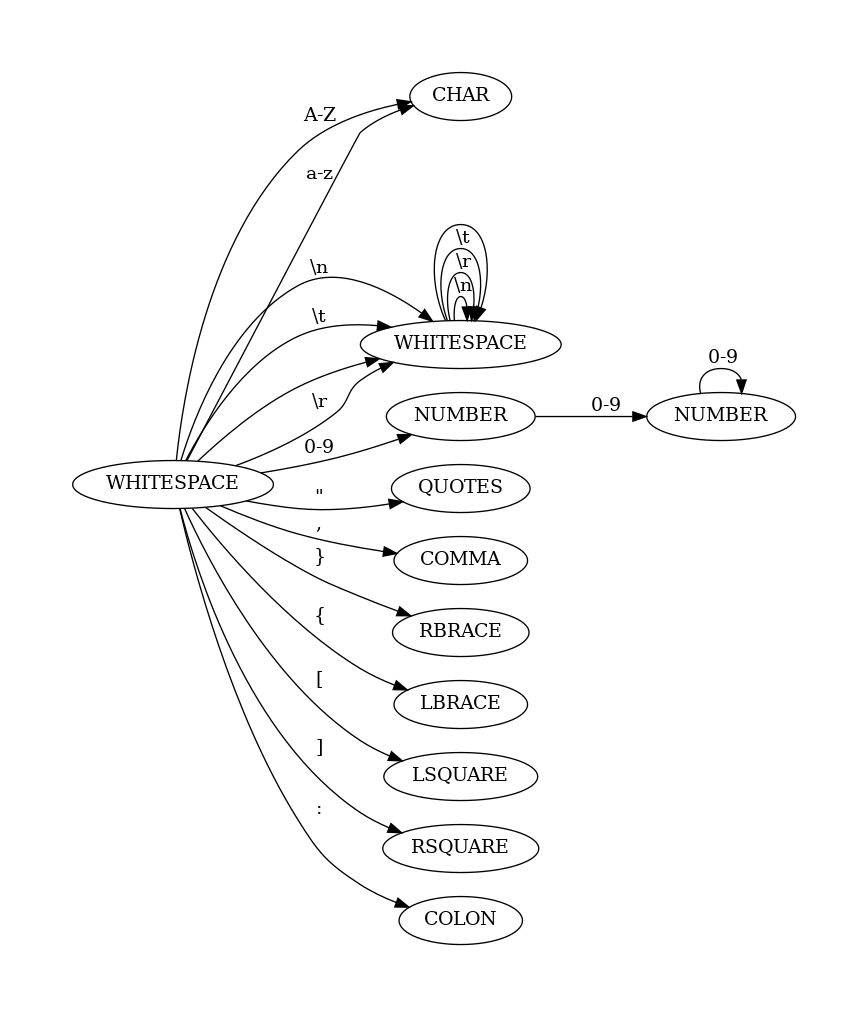
\includegraphics[width=\linewidth]{images/dfa.png}
\caption{DFA of the lexical grammar}
\label{fig:dfa}
\end{figure}

\begin{figure}[t]
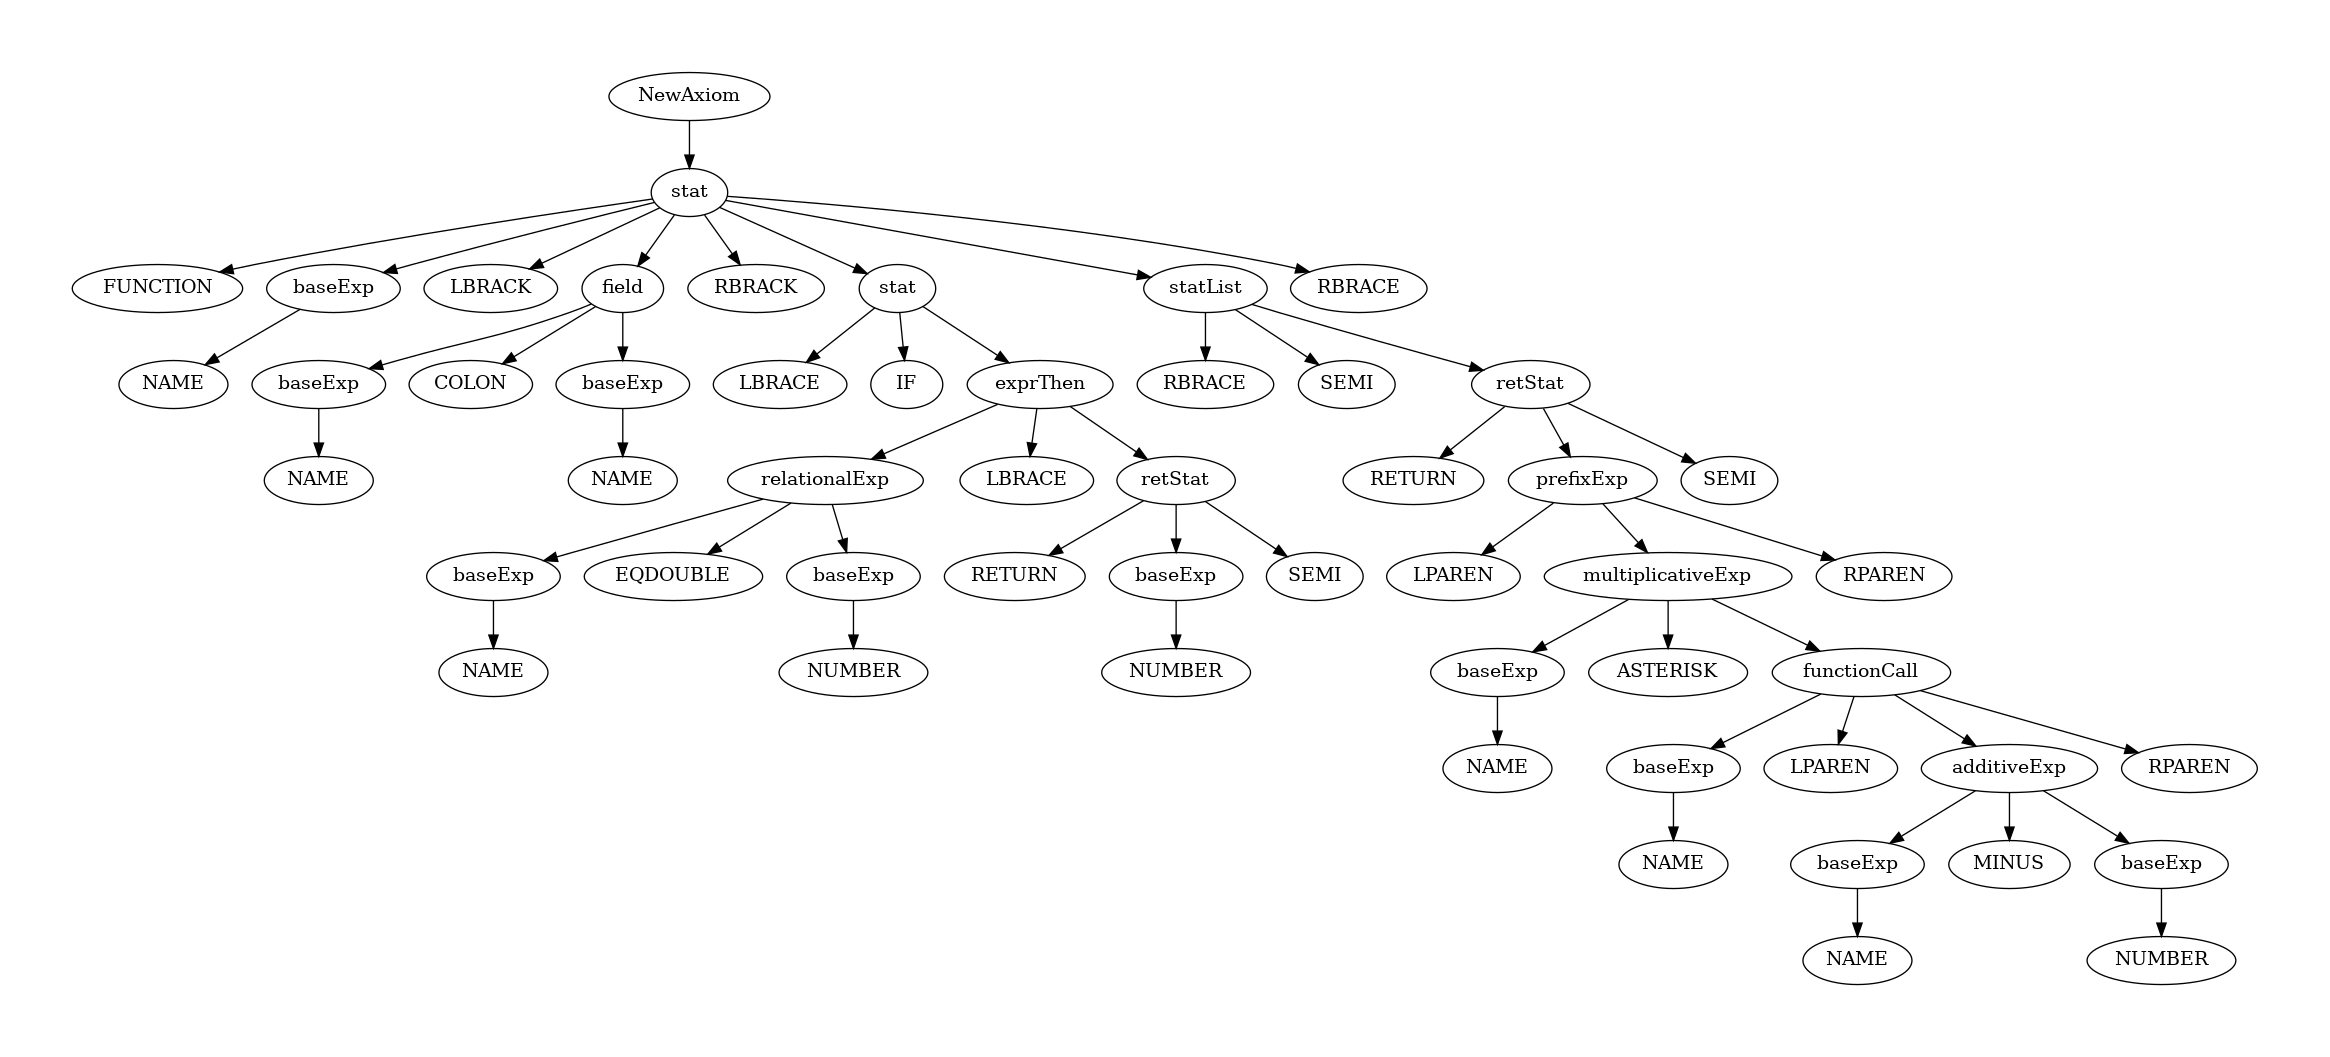
\includegraphics[width=\linewidth]{images/ptree.png}
\caption{Graphviz visualization of the parse tree.}
\label{fig:parse_tree}
\end{figure}

